\begin{pastexam}[label={px:ntu-110-dsaa-13}]{臺大資工所 110 學年度 第 XIII 題}
（單選；每格答對 5 分，答錯倒扣 2.5 分）

The VERTEX-COVER problem is to find a vertex cover of the size $k$ in a given graph $G$. In the
SUBSET-SUM problem, given a finite set $S\subset\mathbf{N}$ and a target $t\in\mathbf{N}$, we ask
whether there is a subset $S'\subseteq S$ whose elements sum to $t$. The VERTEX-COVER problem is
polynomial-time reducible to the SUBSET-SUM problem. Given an instance $<G,k>$ of the
VERTEX-COVER problem, one can construct a corresponding instance $<S,t>$ of the SUBSET-SUM
problem. Given the following graph $G$ and $k=3$, $\{v_1,v_3,v_4\}$ is the vertex cover of size
$k=3$. The corresponding set $S=\{1,4,16,64,256,1040,1041,1093,1284,1344\}$ is constructed as the
following table. What is the target $t$? \underline{\makebox[5em]{(20)}}

(A) 2389 \qquad (B) 3417 \qquad (C) 3754 \qquad (D) 3758

\begin{center}
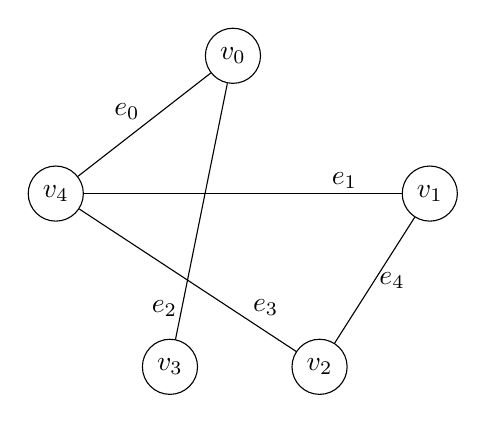
\begin{tikzpicture}[x=1cm,y=1cm,v/.style={circle,draw,inner sep=0pt,minimum size=7mm},w/.style={inner sep=1.5pt}]
\node[v] (v0) at (0,0) {$v_0$};
\node[v] (v4) at (-2.25,-1.75) {$v_4$};
\node[v] (v1) at (2.5,-1.75) {$v_1$};
\node[v] (v3) at (-0.8,-3.95) {$v_3$};
\node[v] (v2) at (1.1,-3.95) {$v_2$};
\draw (v0)--node[w,above left]{$e_0$}(v4);
\draw (v4)--node[w,above,pos=0.82]{$e_1$}(v1);
\draw (v0)--node[w,left,pos=0.88]{$e_2$}(v3);
\draw (v4)--node[w,above right,pos=0.78]{$e_3$}(v2);
\draw (v1)--node[w,right,pos=0.5]{$e_4$}(v2);
\end{tikzpicture}
\end{center}
\begin{center}
\begin{tabular}{ccc|ccccc|cr}
\multicolumn{3}{c}{} & \multicolumn{5}{c}{\textit{modified based 4}} & & \textit{decimal}\\
 & & & $e_4$ & $e_3$ & $e_2$ & $e_1$ & $e_0$ & & \\ \cline{4-8}
$x_0$ & = & 1 & 0 & 0 & 1 & 0 & 1 & = & 1041\\
$x_1$ & = & 1 & 1 & 0 & 0 & 1 & 0 & = & 1284\\
$x_2$ & = & 1 & 1 & 1 & 0 & 0 & 0 & = & 1344\\
$x_3$ & = & 1 & 0 & 0 & 1 & 0 & 0 & = & 1040\\
$x_4$ & = & 1 & 0 & 1 & 0 & 1 & 1 & = & 1093\\ \cline{4-8}
\multicolumn{1}{c}{$y_0$} & = & \multicolumn{1}{c}{0} & 0 & 0 & 0 & 0 & \multicolumn{1}{c}{1} & = & 1\\
\multicolumn{1}{c}{$y_1$} & = & \multicolumn{1}{c}{0} & 0 & 0 & 0 & 1 & \multicolumn{1}{c}{0} & = & 4\\
\multicolumn{1}{c}{$y_2$} & = & \multicolumn{1}{c}{0} & 0 & 0 & 1 & 0 & \multicolumn{1}{c}{0} & = & 16\\
\multicolumn{1}{c}{$y_3$} & = & \multicolumn{1}{c}{0} & 0 & 1 & 0 & 0 & \multicolumn{1}{c}{0} & = & 64\\
\multicolumn{1}{c}{$y_4$} & = & \multicolumn{1}{c}{0} & 1 & 0 & 0 & 0 & \multicolumn{1}{c}{0} & = & 256\\
\end{tabular}
\end{center}
\end{pastexam}

\begin{pastsoln}
答案是 (C) 3754。

\textbf{先讀出構造}。 每個數寫成 $6$ 位的 $4$ 進位數：最左一位在頂點的數 $x_i$ 是 $1$、在邊的數 $y_j$
是 $0$；右邊五位依序對應 $e_4, \ldots, e_0$。 $x_i$ 在 $e_j$ 那一位是 $1$，若且唯若 $e_j$ 碰到 $v_i$；
$y_j$ 只有 $e_j$ 那一位是 $1$。 例如 $v_0$ 碰到 $e_0$、$e_2$，$x_0 = 4^5 + 4^2 + 4^0 = 1024 + 16 + 1 =
1041$，和表上一樣。 對照圖：$e_0 = v_0v_4$、$e_1 = v_4v_1$、$e_2 = v_0v_3$、$e_3 = v_4v_2$、
$e_4 = v_1v_2$，五列 $x_i$ 的 $1$ 都和圖相符。

\textbf{目標}。 最左一位要是 $k$，每個邊的位要是 $2$：
\[
t = k \cdot 4^5 + \sum_{j=0}^{4} 2 \cdot 4^j = 3 \cdot 1024 + 2\,(1 + 4 + 16 + 64 + 256) = 3072 + 682 = 3754.
\]
道理和資結書第~28.5.2~節的十進位構造一樣。 一個邊的位最多有三個 $1$（兩個端點的 $x$ 和 $y_j$），不到
$4$，所以相加不會進位，每一位可以分開看。 最左一位是 $k$，表示恰好挑了 $k$ 個頂點的數。 邊 $e_j$ 的位
要湊到 $2$：挑到的端點有兩個時，不挑 $y_j$；只有一個時，再挑 $y_j$；一個都沒有時，最多只有 $y_j$ 的
$1$，湊不到 $2$。 所以湊得出 $t$ 若且唯若挑出的 $k$ 個頂點蓋住每一條邊。

\textbf{用題目給的覆蓋驗算}。 $x_1 + x_3 + x_4 = 1284 + 1040 + 1093 = 3417$。 各邊被覆蓋
$\{v_1, v_3, v_4\}$ 碰到的次數：$e_0 = \{v_0, v_4\}$ 一次、$e_1 = \{v_4, v_1\}$ 兩次、
$e_2 = \{v_0, v_3\}$ 一次、$e_3 = \{v_4, v_2\}$ 一次、$e_4 = \{v_1, v_2\}$ 一次。 只碰到一次的邊要補
$y_0, y_2, y_3, y_4$：$3417 + 1 + 16 + 64 + 256 = 3754 = t$。

\textbf{其他選項}。 (B) $3417$ 只是三個 $x$ 的和，漏了補上的 $y$；而且目標 $t$ 必須只由 $G$ 和 $k$
決定，不能隨某一個覆蓋改變，否則就是構造時偷看答案。 (A) $2389 = 2 \cdot 4^5 + (1 + 4 + 16 + 64 + 256)$，
是把 $k$ 寫成 $2$、每個邊的位寫成 $1$。 (D) $3758 = 3417 + (1 + 4 + 16 + 64 + 256)$，是三個 $x$ 再加上
全部五個 $y$；$e_1$ 已經被碰到兩次，又多補了 $y_1$，那一位變成 $3$，不是 $2$。
\end{pastsoln}
